\chapter{Link budget}
The link buget was calculated to estimate the link status, whether the selected component are sufficient to "close" the link. A link budget calculates all of the gains and losses in the radio system, estimating the link margin. In the satellite case, the link budget is a valuable tool - because of the direct line of sight between two communicating nodes, most of the parameters are well known and stable throughout the system lifetime. Main gains from the system comes from: output power of the transmitter and the antennas gain, whereas losses include: free space loss, losses through the medium (atmoshperic losses, ionisation lossed), cable and other in-line devices attenuation, polarisation losses and antenna pointing losses. This section provides an description of the PW-Sat2 link budget, which was based on AMSAT/IARU Link Budget \cite{amsat_link_budget}.

\section{Orbit and slant range}
A slant range (fig \ref{slant_range}) is an maximal distance between the spacecraft and the ground station. It is calculated from the Orbit altitude and the minimal elevation required. For PW-Sat2, useful elevation was assumed at \SI{5}{\degree}. Assumed orbital parameters gives maximum slant range of about \SI{2300}{\kilo\meter} (fig. \ref{slant_range_calc}) and period of \SI{96}{\minute}.

\begin{figure}
    \centering
    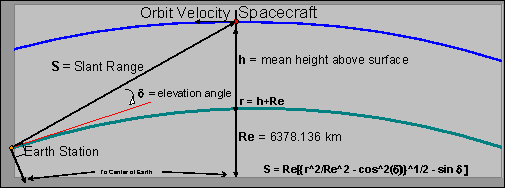
\includegraphics[width=0.8\paperwidth]{img/6/slant_range.pdf}
    \caption{Slant range. Source: \cite{amsat_link_budget}}
    \label{slant_range}
\end{figure}

\begin{figure}
    \centering
    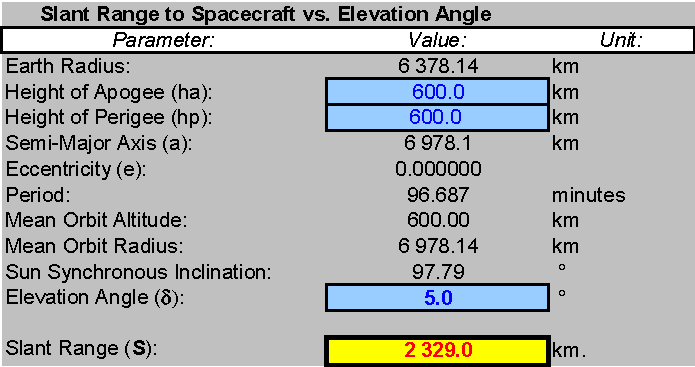
\includegraphics[width=0.8\paperwidth]{img/6/slant_range_calc.pdf}
    \caption{Slant range calculation.}
    \label{slant_range_calc}
\end{figure}

\section{Transmitter capabilities}
The transmitter output power and any in-line losses, as well as antenna mismatch are entered and calculated in the link budget. All the in-line losses are estimated, such as the feeder loss, splitter insertion loss and, if applicable, any other elements, such as the surge protection. The result the power that is actually delivered to the antennas on both the ground station and the spacecraft. The results shown in the figures \ref{link:tx_gs} and \ref{link:tx_spacecraft} indicate the output power \SI{26.63}{\dBm} on the spacecraft and \SI{47.45}{\dBm} on the ground station.

\begin{figure}
    \centering
    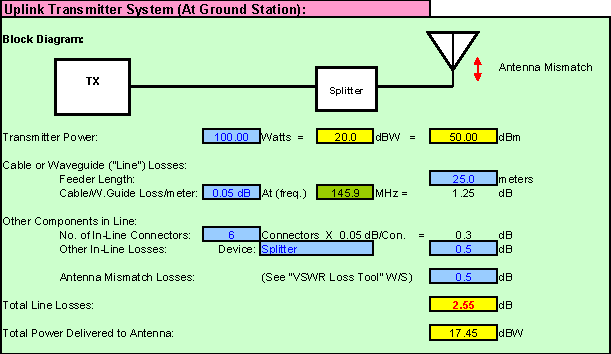
\includegraphics[width=0.8\paperwidth]{img/6/tx_gs.pdf}
    \caption{Ground station output power calculation}
    \label{link:tx_gs}
\end{figure}

\begin{figure}
    \centering
    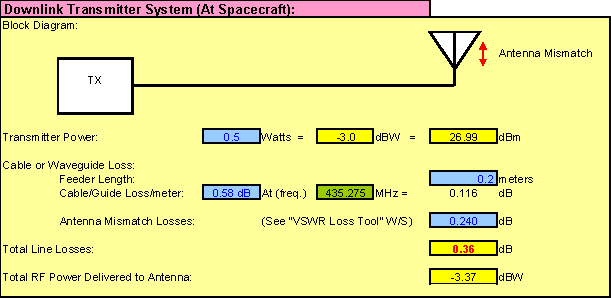
\includegraphics[width=0.8\paperwidth]{img/6/tx_spacecraft.pdf}
    \caption{Spacecraft output power calculation.}
    \label{link:tx_spacecraft}
\end{figure}


\section{Antenna gain}
The antenna gain directly affect the radio link budget. The directional gain of the antennas is taken from the documentation of the manufacturers and for the antennas in the system they are equal to:
\begin{itemize}
    \item Ground station - Cross-Yagi antennas, \SI{13.2}{\dBi} for uplink, \SI{16.2}{\dBi} for downlink,
    \item Spacecraft - both antennas are dipoles, \SI{2.15}{\dBi} as for ideal dipole is assumed as the antennas are working in the resonance. 
\end{itemize}


\section{Medium losses}
The main signal loss in the spacecraft communication comes from the Free space loss, given by the formula: $\text{Loss [dB]} = 22 + 20 \cdot \log_{10} (\text{d}/\lambda)$, where $d$ - distance in meters, $\lambda$ - wavelength. Other sources of losses taken into the consideration for the sub-GHz bands are atmospheric losses and losses in the ionosphere. Atmospheric absorption strongly depends on the total number of molecules along the path between the spacecraft and the ground station - therefore the elevation angle. Losses due to the atmospheric gases are nearly independent of atmospheric temperature, density and relative humidity at frequencies below 2 GHz. \cite{sat_propagation}. At \SI{5}{\degree} elevation, the atmospheric are estimated at \SI{2.1}{\dB}. The ionosphere limits the lowest frequency at which satellite communications is possible. Below \SI{20}{\MHz}, during solar maximum, signals are usually fully absorbed or reflected by the layers of the ionosphere. VHF, UHF and Microwave frequencies are influenced far less amount, but the value of the attenuation varies with time. For the purpose of calculation above \SI{100}{\MHz} is is sufficient to estimate losses in the ionosphere as below \SI{1}{\dB}.

Total medium losses are equal:
\begin{itemize}
    \item Uplink - \SI{145.9}{\MHz} - $FSPL = \SI{146.2}{\dB}$
    \item Downlink - \SI{145.9}{\MHz} - $FSPL = \SI{155.7}{\dB}$
\end{itemize}


\section{Polarization losses}
On the ground station, both antennas has circular polarization, whereas on the spacecraft, antennas are linearly polarized. This eliminates the effect of signal strength variance with the rotation of the satellite, but only the half power is received by the antennas. The polarization loss of \SI{3}{\dB} was assumed in both uplink and downlink.

\section{Antenna pointing losses}
Antenna pointing losses are exhibited when the maximal directivity gain of the antennas are not aligned with the receiver (fig. \ref{link:pointing_loss}). For ground station, the rotator and its controller are pointing with the accuracy of about \SI{1}{\degree} but due to the wind and other non-ideal factors the pointing error was assumed for \SI{5}{\degree}. The antenna gain loss was read from the radiation patterns (fig. \ref{radiation_144} and \ref{radiation_435}) as estimated at \SI{1}{\dB}. For the spacecraft, as the antennas have dipole characteristics, they are mostly omnidirectional, but with significant drops in the directivity along the dipole axis. The communication will break at some angles along the dipole axis, is was assumed that the coverage of \si{300} per \SI{360}{\degree} is sufficient. At standard dipole roll-off factor (fig. \ref{link:dipole_pattern}), \SI{70}{\degree} pointing error equals to \SI{4.7}{\dB} pointing loss.

\begin{figure}
    \centering
    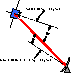
\includegraphics[width=0.5\paperwidth]{img/6/pointing_loss.pdf}
    \caption{Pointing losses. Source: \cite{amsat_link_budget}}
    \label{link:pointing_loss}
\end{figure}

\begin{figure}
    \centering
    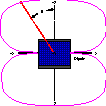
\includegraphics[width=0.4\paperwidth]{img/6/dipole_pattern.pdf}
    \caption{Dipole antenna radiation pattern. Source: \cite{amsat_link_budget}}
    \label{link:dipole_pattern}
\end{figure}


\section{Antenna temperature}
For receiver antennas the antenna temperature is the total noise figure added by the antenna which come from other sources than transmitter of interest. It adds to the noise produced by the Low Noise Amplifier, resuling in lowering the Signal To Noise ratio.
The sky temperature as seen by a spacecraft must be viewed from its perspective. In the beamwidth of the omnidirectional antenna on Low Earth Orbit there is a half of a sphere of the deep space and half of the Earth. The sky itself which is nominally at \SI{2.7}{\kelvin} but, at frequencies below \SI{2}{\GHz} also includes galactic noise, which is highest in directions that intercept the disk of the Milky Way.  At \SI{146}{\MHz} this value can be as high as \SI{1700}{\kelvin} and as low as \SI{80}{\kelvin} \cite{amsat_link_budget}. The average Earth temperature used is \SI{290}{\kelvin}, however, the Earth may be warmer due to man-made noise sources that can be distributed on the surface of the planet. The average antenna temperature of the spacecraft was assumed to $0.5 \cdot \SI{70}{\kelvin} + 0.5 \cdot \SI{330}{\kelvin} = \SI{200}{\kelvin}$.
For a ground station antenna the Sky Temperature value must include not only the noise intercepted by the ground station antenna coming from the colder sky into which the antenna is looking but, it has to include any terrestrially generated noise that may be generated in the proximity of the station. This condition is worst when the ground station antenna is at low elevation angles and pointed in the direction of the source of the noise. For PW-Sat2, the receiver antenna is placed in the middle of the Warsaw, resulting in increased temperature depending on the azimuth of the antenna. During ground station calibration, the power spectrum density was measured using spectrum analyzer, resulting in the noise floor of about \SI{-132}{\dBm} in \SI{10}{\kHz} RBW. This implies the antenna temperature of about \SI{500}{\kelvin}.


\section{Receiver performance}
The receiver performance was measured for both uplink and downlink using the attenuators and packet transmitters. During the sensitivity tests, the "effective" antenna temperature was \SI{290}{\kelvin} - the noise was produced by the electrical components in the room temperature. This means that during the mission, the sensitivity will be affected by the noise added by the antenna.
For uplink, the effective sky antenna (\SI{200}{\kelvin}) is actually lower then the room temperature, meaning that the sensitivity of the system will improve by $10\cdot \log_{10}(200/290) = \SI{1.6}{\dB}$, resulting in receiver sensitivity for \SI{1}{\percent} PER: \SI{-98}{\dBm}.
In the ground station the effective antenna temperature will be higher than during tests on the bench, resulting in the reduce of the sensitivity by $\SI{2.3}{\dB}$. This gives the effective sensitivity at \SI{-124}{\dBm}.


\section{Link budget summary}
Summing all the gains and losses produces a valuable overview of the system performance (fig. \ref{link:link_status}). The power on the receiver ports of the system are calculated and compared to the sensitivities of the receivers, resulting in link status and margin. The link margins are above \SI{5}{\dB} - the safe limit and are equal to \SI{6.0}{\dB} for downlink and \SI{5.7}{\dB} for uplink. Most of the time the performance will be better due to the lower pointing losses of the spacecraft. 

\begin{figure}
    \centering
    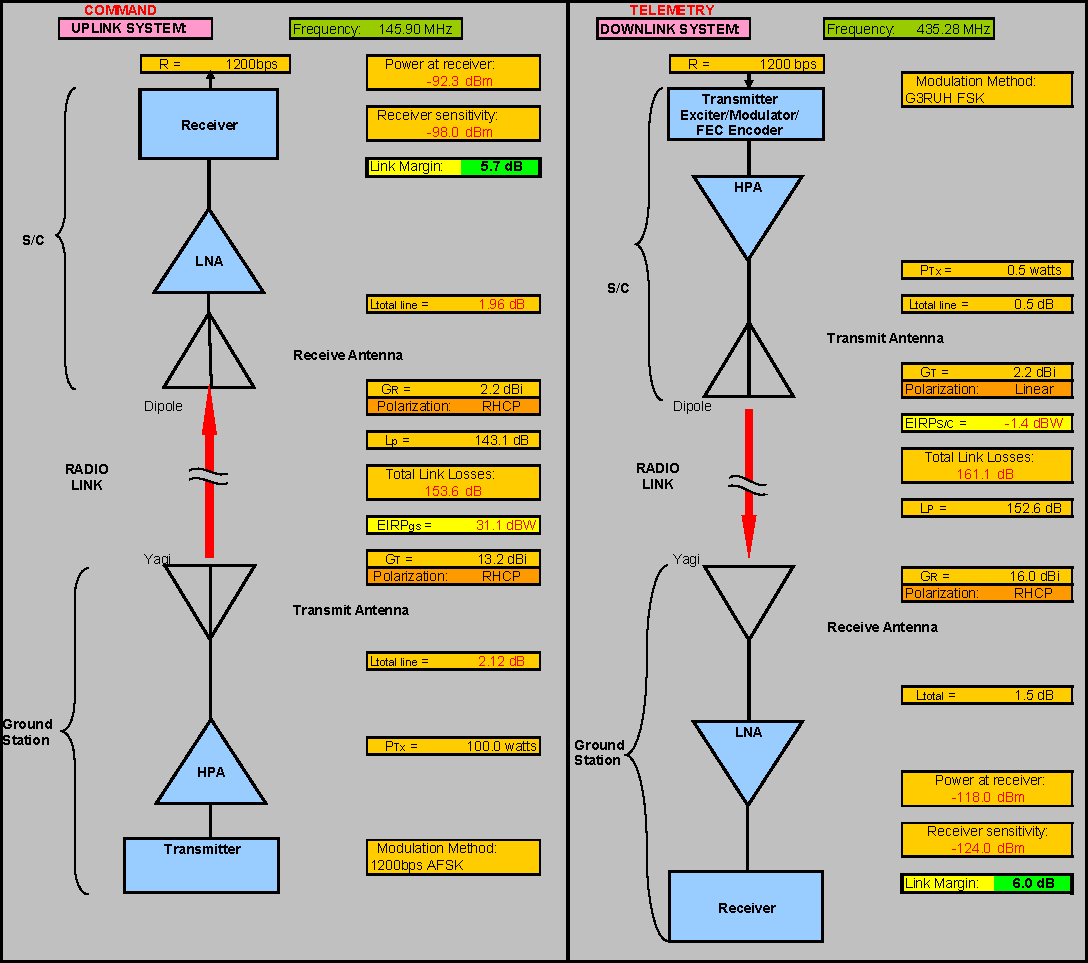
\includegraphics[width=0.8\paperwidth]{img/6/link_summary.pdf}
    \caption{System performance summary.}
    \label{link:link_status}
\end{figure}